\subsection{作业 5}

\begin{homework}
    现有信号 $f(t) = \mathe^{-t^2/20}$。为分析某时刻下的``局部频谱'',
    可选合适的窗函数 $w(t, t_0)$,并截取 $f(t)$ 在 $t_0$ 附近的信号,
    即 $f_w(t, t_0) = f(t)\cdot w(t, t_0)$。
    \begin{enumerate}[label=(\arabic*)]
        \item 求信号 $f(t)$ 的 FT。
        \item 现不妨取窗函数 $w(t, t_0) = \mathe^{-(t - t_0)^2/2}$。
            试分析 $t_0 = 0$ 时刻下对应的``局部频谱'',即求 $f_w(t, 0)$ 的 FT。
        \item 画出信号 $f(t)$ 的频谱图与信号 $f(t)$ 在 $t_0 = 0$ 时刻下的
            ``局部频谱''图,并进行对比。
    \end{enumerate}
    (提示:若 $x, c \in \set{R}$,则 $\int_{-\infty}^{+\infty}\mathe^{-(x + \mathi c)^2}\D{x} = \sqrt{\pi}$。)
\end{homework}

\begin{solution}
    \begin{enumerate}[label=(\arabic*)]
        \item 不妨记 $f(t)$ 的 FT 为 $F(\omega)$。由傅里叶变换的定义知
            \begin{align*}
                F(\omega) & = \mathcal{F}[f(t)] = \int_{-\infty}^{+\infty} f(t)\mathe^{-\mathi\omega t}\D{t} \\
                & = \int_{-\infty}^{+\infty} \mathe^{-t^2/20}\mathe^{-\mathi\omega t}\D{t} \\
                & = \mathe^{-5\omega^2}\int_{-\infty}^{+\infty} \mathe^{-\frac{(t + 10\mathi \omega)^2}{20}}\D{t} \\
                & = 2\sqrt{5\pi}\mathe^{-5\omega^2}.
            \end{align*}
        \item 不妨记 $f_w(t, 0)$ 的 FT 为 $F_w(\omega, 0)$。由题知
            \begin{align*}
                f_w(t, 0) = f(t)\cdot w(t, 0) = \mathe^{-t^2/20}\mathe^{-t^2/2} = \mathe^{-\frac{11}{20}t^2}.
            \end{align*}
            因此,其傅里叶变换为
            \begin{align*}
                F_w(\omega, 0) & = \mathcal{F}[f_w(t, 0)] = \int_{-\infty}^{+\infty} f_w(t, 0)\mathe^{-\mathi\omega t}\D{t} \\
                & = \int_{-\infty}^{+\infty} \mathe^{-\frac{11}{20}t^2}\mathe^{-\mathi\omega t}\D{t} \\
                & = \mathe^{-\frac{5}{11}\omega^2}\int_{-\infty}^{+\infty} \mathe^{-\frac{11}{20}\left(t + \frac{10}{11}\mathi \omega\right)^2}\D{t} \\
                & = \frac{2}{11}\sqrt{55\pi}\mathe^{-\frac{5}{11}\omega^2}.
            \end{align*}
        \item 画出两者的频谱图如 \ref{fig:chap2-part6-exercise1-solution} 所示。
            \begin{figure}[H]
                \centering
                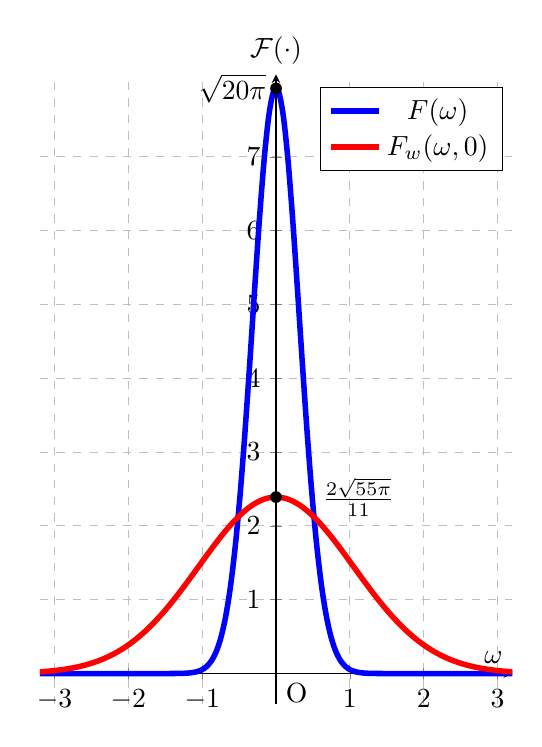
\begin{tikzpicture}
                    \begin{axis}[
                        axis lines = middle,
                        xlabel = {$\omega$},
                        ylabel = {$\mathcal{F}(\cdot)$},
                        ylabel style={at={(rel axis cs:0.5, 1)}, anchor=south},
                        xmin = -3.2, xmax = 3.2,
                        ymin = -0.2, ymax = 7.9,
                        xtick distance = 1,
                        ytick = {1, 2, 3, 4, 5, 6, 7},
                        grid = major,
                        grid style = dashed,
                        scale only axis,
                        width = 6cm,
                        height = 8cm,
                        axis equal,
                    ]
                    \addplot[domain=-3.2:3.2, samples=100, smooth, line width=2pt, blue] {sqrt(20 * pi) * exp(-5 * x^2)};
                    \addlegendentry{$F(\omega)$}
                    \addplot[domain=-3.2:3.2, samples=100, smooth, line width=2pt, red] {sqrt(20 / 11 * pi) * exp(-5 / 11 * x^2)};
                    \addlegendentry{$F_w(\omega, 0)$}
                    \node at (axis cs:0, 0) [anchor=north west] {O};
                    \node[circle, fill, inner sep=1.5pt] at (axis cs:0, 7.927) {};
                    \node at (axis cs:0, 7.927) [anchor=east] {$\sqrt{20\pi}$};
                    \node[circle, fill, inner sep=1.5pt] at (axis cs:0, 2.390) {};
                    \node at (axis cs:0.5, 2.390) [anchor=west] {$\frac{2\sqrt{55\pi}}{11}$};
                    \end{axis}
                \end{tikzpicture}
                \caption{频谱图像对比}
                \label{fig:chap2-part6-exercise1-solution}
            \end{figure}
            可以看出,这两个频率谱在 $\omega = 0$ 处均有峰值,但 $F(\omega)$ 的峰值更高,
            为 $F_w(\omega, 0)$ 的 $\sqrt{11}$ 倍。同时,$F_w(\omega, 0)$ 比 $F(\omega)$ 更加
            ``平缓'',即 $F_w(\omega, 0)$ 的峰值附近的值相对于峰值更小。
    \end{enumerate}
\end{solution}
